%%%%%%%%%%%%%%%%%%%%%%%%%%%%%%%%%%%%%%%%%
% Beamer Presentation
% LaTeX Template
% Version 1.0 (10/11/12)
%
% This template has been downloaded from:
% http://www.LaTeXTemplates.com
%
% License:
% CC BY-NC-SA 3.0 (http://creativecommons.org/licenses/by-nc-sa/3.0/)
%
%%%%%%%%%%%%%%%%%%%%%%%%%%%%%%%%%%%%%%%%%

%----------------------------------------------------------------------------------------
%	PACKAGES AND THEMES
%----------------------------------------------------------------------------------------

\documentclass[xcolor=table]{beamer}

\mode<presentation> {

% The Beamer class comes with a number of default slide themes
% which change the colors and layouts of slides. Below this is a list
% of all the themes, uncomment each in turn to see what they look like.

\usetheme{default}
%\usetheme{AnnArbor}
%\usetheme{Antibes}
%\usetheme{Bergen}
%\usetheme{Berkeley}
%\usetheme{Berlin}
%\usetheme{Boadilla}
%\usetheme{CambridgeUS}
%\usetheme{Copenhagen}
%\usetheme{Darmstadt}
%\usetheme{Dresden}
%\usetheme{Frankfurt}
%\usetheme{Goettingen}
%\usetheme{Hannover}
%\usetheme{Ilmenau}
%\usetheme{JuanLesPins}
%\usetheme{Luebeck}
%\usetheme{Madrid}
%\usetheme{Malmoe}
%\usetheme{Marburg}
%\usetheme{Montpellier}
%\usetheme{PaloAlto}
%\usetheme{Pittsburgh}
%\usetheme{Rochester}
%\usetheme{Singapore}
%\usetheme{Szeged}
%\usetheme{Warsaw}

% As well as themes, the Beamer class has a number of color themes
% for any slide theme. Uncomment each of these in turn to see how it
% changes the colors of your current slide theme.

%\usecolortheme{albatross}
%\usecolortheme{beaver}
%\usecolortheme{beetle}
%\usecolortheme{crane}
%\usecolortheme{dolphin}
%\usecolortheme{dove}
%\usecolortheme{fly}
%\usecolortheme{lily}
%\usecolortheme{orchid}
%\usecolortheme{rose}
%\usecolortheme{seagull}
%\usecolortheme{seahorse}
%\usecolortheme{whale}
%\usecolortheme{wolverine}
%\setbeamertemplate{footline} % To remove the footer line in all slides uncomment this line
\setbeamertemplate{footline}[page number] % To replace the footer line in all slides with a simple slide count uncomment this line

\setbeamertemplate{navigation symbols}{} % To remove the navigation symbols from the bottom of all slides uncomment this line 
}
\usepackage{graphicx} % Allows including images
\usepackage{booktabs} % Allows the use of \toprule, \midrule and \bottomrule in tables
\usepackage[table]{xcolor}
\usepackage{pgfplots}
\usepackage{tcolorbox}
\pgfplotsset{compat=1.15}
\usepackage{mathrsfs}
\usetikzlibrary{arrows}
\usetikzlibrary{patterns}


\usepackage{tikz}
\usepackage{pstricks-add}
\usetikzlibrary{arrows,shapes,positioning,shadows,trees}


\usepackage{tcolorbox}
\usepackage{wrapfig}


\usepackage{hyperref}
\hypersetup{
    colorlinks,
    citecolor=black,
    filecolor=black,
    linkcolor=black,
    urlcolor=black
}
\newcommand{\notimplies}{%
    \mathrel{{\ooalign{\hidewidth$\not\phantom{=}$\hidewidth\cr$\implies$}}}}


\DeclareMathAlphabet\mathzapf{T1}{pzc}{mb}{it}
\usepackage{amsmath,wasysym}
\usepackage{latexsym}

\usepackage{amssymb}
\usepackage{mathrsfs}
\usepackage{bm}
\usepackage{wrapfig}
\usepackage{fancybox}
\bibliographystyle{amsplain}
\usepackage{systeme}
\usepackage{pdfpages}

\usepackage{latexsym}
\usepackage{graphicx}


\usepackage{yfonts}
\usepackage[french]{babel}



\usepackage[T2A]{fontenc}




%\usepackage[style=ieee]{biblatex} %Use if necessary for citation
%\addbibresource{biblatex-examples.bib}
%----------------------------------------------------------------------------------------
%	TITLE PAGE
%----------------------------------------------------------------------------------------

\title[Physique]{Mathématiques I} % The short title appears at the bottom of every slide, the full title is only on the title page

\author{Team Physique} % Your name
\institute[S4S] % Your institution as it will appear on the bottom of every slide, may be shorthand to save space
{
Initiative Students4Students\\ % Your institution for the title page
\medskip
}
\date{\today} % Date, can be changed to a custom date

\begin{document}
\begin{frame}
\titlepage % Print the title page as the first slide
\end{frame}

%\begin{frame}{Présentation} %4'
%    \begin{itemize}
%        \item Présentation des speakers et de l'équipe
%        \item But de S4S et de ce cours de Physique
%        \item Cas spéciaux: AR et PH
        %\item Format du cours
    
    %\end{itemize}
%\end{frame}
    

\begin{frame}{Mécanique - Imaginer le mouvement d'un objet} % 3'
    \begin{figure}[h]
    \centering
    \begin{center}
    
\definecolor{rvwvcq}{rgb}{0.08235294117647059,0.396078431372549,0.7529411764705882}
\begin{tikzpicture}[line cap=round,line join=round,>=triangle 45,x=2.077922077922078cm,y=2.6086956521739126cm]
\begin{axis}[
x=2.077922077922078cm,y=2.6086956521739126cm,
axis lines=middle,
ymajorgrids=true,
xmajorgrids=true,
xmin=-0.05,
xmax=3.8,
ymin=-0.05,
ymax=1.1,
xtick={-0.0,0.5,...,3.5},
ytick={-0.0,0.5,1.0},]
\clip(-0.05,-0.05) rectangle (3.8,1.1);
\draw[line width=4.pt] (-0.086090907575987,1.6578211468632087) -- (0.49556511308165885,1.6578211468632087);
\draw[line width=4.pt] (-0.35074439697521587,1.7567026703750082) -- (0.23091162368243,1.7567026703750082);
\begin{scriptsize}
\draw [fill=black] (0.08840589862130677,1.6578211468632087) circle (2.5pt);
\draw[color=black] (0.10003901903445966,1.726165729290482) node {$t = 3$};
\draw [fill=black] (-0.187880711191075,1.7567026703750082) circle (2.5pt);
\draw[color=black] (-0.14134822953846338,1.8250472528022814) node {$v0 = -5.8$};
\draw [fill=rvwvcq] (3.,0.5921521997621881) circle (2.5pt);
\draw[color=rvwvcq] (3.1,0.7) node {$P$};
\draw[color=black] (3.55,0.1) node {$x(t)$};
\draw[color=black] (0.2,1.025) node {$y(t)$};
\draw [fill=rvwvcq] (0.1,0.09732461355529132) circle (2.5pt);
\draw [fill=rvwvcq] (0.3,0.2759215219976218) circle (2.5pt);
\draw [fill=rvwvcq] (0.4,0.3571938168846611) circle (2.5pt);
\draw [fill=rvwvcq] (0.5,0.43311533888228293) circle (2.5pt);
\draw [fill=rvwvcq] (0.6,0.5036860879904874) circle (2.5pt);
\draw [fill=rvwvcq] (0.7,0.5689060642092746) circle (2.5pt);
\draw [fill=rvwvcq] (1.,0.7324613555291319) circle (2.5pt);
\draw [fill=rvwvcq] (1.1,0.7762782401902496) circle (2.5pt);
\draw [fill=rvwvcq] (1.4,0.8756242568370985) circle (2.5pt);
\draw [fill=rvwvcq] (1.6,0.9151010701545779) circle (2.5pt);
\draw [fill=rvwvcq] (1.7,0.9268133174791915) circle (2.5pt);
\draw [fill=rvwvcq] (1.9,0.9341854934601663) circle (2.5pt);
\draw [fill=rvwvcq] (2.3,0.8847205707491081) circle (2.5pt);
\draw [fill=rvwvcq] (2.4,0.8589774078478003) circle (2.5pt);
\draw [fill=rvwvcq] (2.5,0.8278834720570747) circle (2.5pt);
\draw [fill=rvwvcq] (2.8,0.7024970273483948) circle (2.5pt);
\draw [fill=rvwvcq] (2.9,0.65) circle (2.5pt);
\draw [fill=rvwvcq] (3.,0.5921521997621881) circle (2.5pt);
\end{scriptsize}
\end{axis}
\end{tikzpicture}
\end{center}

    \caption{La position d'un projectile est une fonction du temps}
    \label{fig:xt}
\end{figure}
\begin{itemize}
    \item La position d'un objet peut être décrite. Et sa vitesse ?
\end{itemize}

\end{frame}

\begin{frame}{La dérivée comme vitesse instantanée}
    \begin{figure}
    \centering

\definecolor{qqwuqq}{rgb}{0,0.39215686274509803,0}
\definecolor{qqqqff}{rgb}{0,0,1}
\definecolor{ccqqqq}{rgb}{0.8,0,0}
\begin{tikzpicture}[line cap=round,line join=round,>=triangle 45,x=1cm,y=1cm]
\begin{axis}[
x=0.75cm,y=0.75cm,
axis lines=middle,
xmin=-1,
xmax=8.385055628710091,
ymin=-1.4004451090161362,
ymax=5.386008244213317,
xtick={-3,-2,...,8},
ytick={-1,-0,...,5},]
\clip(-1,-1.4004451090161362) rectangle (8.385055628710091,5.386008244213317);
\draw [shift={(1.9833804,-0.1)},line width=1.2pt]  plot[domain=1.1705556697609223:2.527573616581852,variable=\t]({1*2.5368001936194266*cos(\t r)+0*2.5368001936194266*sin(\t r)},{0*2.5368001936194266*cos(\t r)+1*2.5368001936194266*sin(\t r)});
\draw [->,line width=0.8pt,color=ccqqqq] (0,0) -- (1.8083053066921226,3.5480972786760643);
\draw [->,line width=0.8pt,color=qqqqff] (0,0) -- (3.493475720586349,3.8426391465182914);
\draw [->,line width=0.8pt,color=qqwuqq] (1.8083053066921226,3.5480972786760643) -- (3.493475720586349,3.8426391465182914);
\begin{scriptsize}
\draw[color=black] (2.437137873052433,3.9683145856067447) node {$\Gamma$};
\draw[color=ccqqqq] (0.55,2.0567376724981345) node {$\vec{r}(t)$};
\draw[color=qqqqff] (3,1.9359316965767727) node {$\vec{r}(t+\Delta t)$};
\draw[color=qqwuqq] (2.350837615096068,3.413002891720386) node {$\vec{d}$};
\end{scriptsize}
\end{axis}
\end{tikzpicture}
    \caption{Vecteur déplacement et intuition derrière la dérivée vectorielle}
    \label{fig:deriveeVect}
\end{figure}
\begin{tcolorbox}[title=Notation des dérivées temporelles, enlarge top by=-1mm, enlarge bottom by=1mm]
\[
    \lim_{\Delta t \to 0} \frac{x(t + \Delta t) - x(t)}{\Delta t} = \frac{dx}{dt}(t) = \dot{x}(t) = x'(t)
\]
\end{tcolorbox}
\end{frame}

\begin{frame}{Intégrales}
   
    
    pas de slides là-dessus, faire intéragir l'audience en jouant un peu avec la notion de primitive (avec les questions écrites dans le doc)
\end{frame}

\begin{frame}{Décomposition d'un vecteur}
\begin{figure}[h]
\begin{center}
\definecolor{ffzzqq}{rgb}{1,0.6,0}
\definecolor{qqqqff}{rgb}{0,0,1}
\definecolor{ffqqqq}{rgb}{1,0,0}
\definecolor{uuuuuu}{rgb}{0.26666666666666666,0.26666666666666666,0.26666666666666666}
\begin{tikzpicture}[line cap=round,line join=round,>=triangle 45,x=1cm,y=1cm]
\begin{axis}[
x=1cm,y=1cm,
axis lines=middle,
xmin=-1.1821895493954007,
xmax=8.455900440737476,
ymin=-2.3726406540327187,
ymax=4.998307713421168,
xtick={-1,0,...,8},
ytick={-2,-1,...,4},]
\clip(-1.1821895493954007,-2.3726406540327187) rectangle (8.455900440737476,4.998307713421168);
\draw [->,line width=1.2pt,color=ffqqqq] (0,0) -- (3.35571,3.23601);
\draw [->,line width=1.2pt,color=qqqqff] (0,0) -- (6.984054440553234,2.1760419327496505);
\draw [->,line width=1.2pt,color=ffzzqq] (3.96723,1.19761) -- (3.35571,3.23601);
\draw [->,line width=1.2pt,color=ffzzqq] (0,0) -- (3.96723,1.19761);
\begin{scriptsize}
\draw [fill=uuuuuu] (0,0) circle (2pt);
\draw[color=ffqqqq] (1.5873326976668879,1.8837856542120805) node {$\vec{a}$};
\draw[color=qqqqff] (5.0000000000000001,1.2690240297390751) node {$\vec{b}$};
\draw[color=ffzzqq] (3.8847125080196666,2.3642615286178104) node {$a_\bot$};
\draw[color=ffzzqq] (2.0378086973080833,0.8590242802100065) node {$a_\parallel$};
\end{scriptsize}
\end{axis}
\end{tikzpicture}
\end{center}
\caption{Décomposition du vecteur $\vec{a}$ par rapport au vecteur $\vec{b}$}
    \label{fig:polar}
\end{figure}

\end{frame}
\begin{frame}{Produit scalaire}

\begin{tcolorbox}[title=Calcul de produit scalaire, enlarge top by=1mm, enlarge bottom by=1mm]
 Soient deux vecteurs dans l'espace $\vec{a} = (a_1, a_2, a_3) $ et $\vec{b} = (b_1, b_2, b_3)$ et $\alpha$ l'angle entre eux. Alors leur produit scalaire vaut : \[ \vec{a} \cdot \vec{b} = a_1 b_1 + a_2 b_2 + a_3 c_3 = \lVert \vec{a} \rVert \lVert \vec{b} \rVert \cos(\alpha)\]

\end{tcolorbox}
 \begin{itemize}
     \item Lien entre la deuxième expression et celle vue en algèbre linéaire ?
 \end{itemize}
\end{frame}
\begin{frame}{Produit vectoriel}
\begin{center}
\begin{tikzpicture} %[scale=1.2, every node/.style={scale=1.2}]
   \draw[-,fill=white!95!red](0,0)--(3,0)--(4,1)--(1,1)--cycle;
\node at (2,0.5) {$\lVert \vec{a} \times \vec{b} \rVert$};
\draw[line width=1.2pt,-latex,blue](0,0)--(3,0)node[midway,below]{$\vec{a}$};
\draw[line width=1.2pt,-latex,red](0,0)--(1,1)node[midway,above]{$\vec{b}$};
\draw[line width=1.0pt,-latex,green](0,0)--(0,3)node[pos=0.7,right]{$\vec{c} = \vec{a} \times \vec{b}$};
\draw (0.6,0) arc [start angle=0,end angle=45,radius=0.6]
node[pos=0.7,right]{$\theta$};
\end{tikzpicture}
%
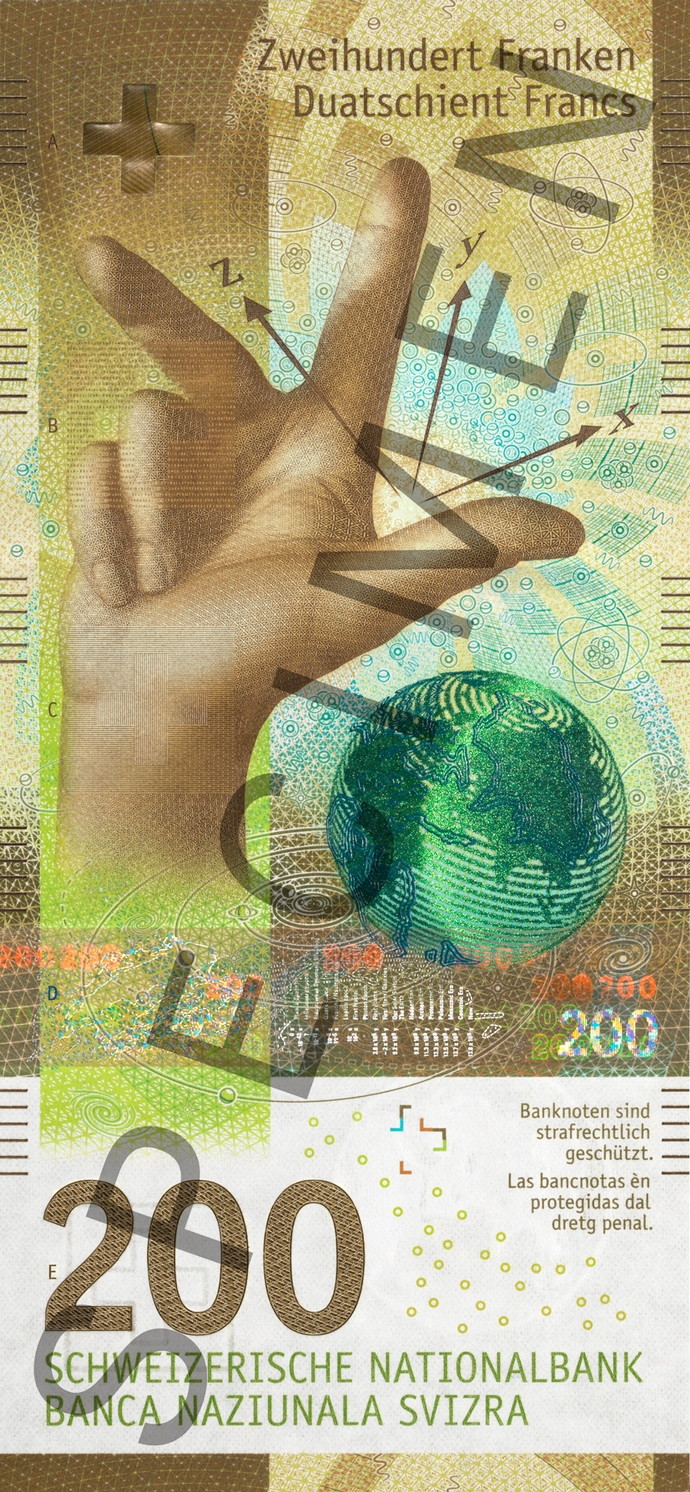
\includegraphics[width=0.15\textwidth]{Images/billet_200.jpg}
\end{center}
\begin{itemize}
    \item Quel est le lien entre ces deux images ? 
    \item Un moyen mnémotechnique important
\end{itemize}
\end{frame}
\begin{frame}{Projection et théorème de Thalès}
    \begin{figure}
    \definecolor{ffqqqq}{rgb}{1,0,0}

    \begin{center}
        
    \begin{tikzpicture}[line cap=round,line join=round,>=triangle 45,x=0.75cm,y=0.75cm]

\begin{axis}[
x=3cm,y=3cm,
axis lines=middle,
xmin=-0.5142915773407036,
xmax=2.181198209028875,
ymin=-0.39259802589438797,
ymax=1.6688390493632528,
xtick={-0.0},
ytick={-0.0},]
\clip(-0.5142915773407036,-0.39259802589438797) rectangle (2.181198209028875,1.6688390493632528);
\draw [->,line width=1.2pt] (0,0) -- (1,0);
\draw [->,line width=1.2pt] (0,0) -- (0,1);
\draw [->,line width=2pt,color=ffqqqq] (0,0) -- (1.5,1.2);
\draw [line width=0.4pt] (0,0) circle (3cm);
\draw [line width=0.8pt] (1.5,1.2)-- (1.5,0);
\draw [line width=0.8pt] (1.5,1.2)-- (0,1.185711555344861);
\draw [line width=0.8pt] (0.7804878048780488,0.624390243902439)-- (0.78,0);
\draw [line width=0.8pt] (0,0.62)-- (0.7804878048780488,0.624390243902439);
\draw (0.6457929204990373,-0.04841070846721544) node[anchor=north west] {$\cos{\alpha}$};
\draw (-0.327101962415107,0.7018961917741242) node[anchor=north west] {$\sin{\alpha}$};
\begin{scriptsize}
\draw[color=black] (0.5179584885758282,0.0822658755554778) node {$\vec{e}_x$};
\draw[color=black] (0.07624777596115196,0.5370396447455734) node {$\vec{e}_y$};
\draw[color=ffqqqq] (0.8671469381737054,0.7698319444774911) node {$\vec{r}$};
\draw[color=black] (1.65,0.6289313420081725) node {$r_y$};
\draw[color=black] (0.7721921843356863,1.2629840531201064) node {$r_x$};
\draw[color=black] (2.1,0.05) node {$x$};
\draw[color=black] (0.05,1.56) node {$y$};

\end{scriptsize}
\end{axis}
\end{tikzpicture}

\end{center}

\caption{Projection du vecteur $\Vec{r}$ sur un repère orthonormé}
    \label{fig:proj}
\end{figure}
\begin{itemize}
    \item $\frac{1}{r} = \frac{\cos{\alpha}}{r_x} = \frac{\sin{\alpha}}{r_y}$
\end{itemize}
\end{frame}
\end{document}